\section{Physikalische Grundlagen}

\subsection{Das Prinzip des Lasers}
Der Begriff des Lasers (Light Amplification by stimulated Emission of Radiation) geht bis auf die  Physiker Schawalow und Townes im Jahre  1958 zurück. Diese stellten Überlegungen an, wie man den bis dahin  bekannten Maser (microwave amplification) auf den optischen Spektralbereich ausdehnen könnte. Heutzutage ist der Laser ein in der  Wissenschaft nicht mehr wegzudenkendes Instrument der Initiierung,  Messung und Steuerung komplexer Prozesse.

\subsection{Emission und Absorption}
Die Elektronen von Atomen befinden sich im Grundzustand alle im energetisch günstigsten Zustand $E_!$. Durch  Energiezufuhr können diese  in energetisch höhere Zustände $E_2$ angeregt werden. Dabei muss die zugeführte Energie genau der Energiedifferenz zwischen den Zuständen entsprechen: $E_2 = E_1 +h\nu$.Man spricht  von gequantelter Absorption. Umgekehrt kann ein Elektron aus einem höheren Zustand durch  Abgabe von Energie in einen unbesetzten niedrigeren Zustand übergehen.  Dabei wird  dann entsprechend  ein Photon mit der Übergangsenergie emittiert.

\subsection{Die Einsteinkoeffizienten}
Albert Einstein führte 1916 drei Koeffizienten zur Beschreibung der Emission und der Absorption ein:

\begin{tabular}{l l}
$B_{12}$ & Beschreibt die Absorption, also die Anregung des Atoms durch ein Photon der Energie $h\nu$ \\
& in einen energetisch höheren Zustand.\\
$B_{21}$ & Beschreibt die stimulierte Emission. Hierbei befindet sich das Atom in einem angeregten Zustand. \\
& Durch eintreffen eines Photons wird eine Relaxion in das niedriger Niveau bewirkt. Durch diesen\\
&  Übergang wird ein Photon erzeugt, welches die selbe Energie wie das eintreffende hat.\\
$A_{21}$ & beschreibt die spontane Emission: Das angeregte Atom relaxiert dabei spontan in ein niedrigeres\\
& Energieniveau, wobei wieder  ein Photon emittiert wird.
\end{tabular}

Über diese Koeffizienten kann nun Berechnet werden, wie viele Atome pro Zeit in einem Strahlungsfeld der Energiedichte $\omega_{\nu}$,  durch Absorption in einen höheren Zustand übergehen:

\begin{equation}
\frac{dN_1}{dt}=-N_1 \cdot B_{12} \cdot \omega_{\nu} + N_2 \cdot B_{21} \cdot \omega_{\nu} + N_2 \cdot A_{21}
\end{equation}

Die Übergangsrate des umgekehrten Übergangs (unter Emission eines Photons) ergibt sich genau umgekehrt:

\begin{equation}
\frac{dN_1}{dt}= N_1 \cdot B_{12} \cdot \omega_{\nu} - N_2 \cdot B_{21} \cdot \omega_{\nu} - N_2 \cdot A_{21}
\end{equation}

Im thermodynamischen Gleichgewicht ist  die Absorption gleich der Emission,sodass die Besetzungszahlen der Zustände der Boltzmann-Verteilung folgen. Da unsere Zustände entartet sein können, muss dies als zusätzliche Gewichtung $g=(2J+1)$ in die Verteilung mit einfließen:

\begin{equation}
\frac{N_1}{N_2} = \frac{g_1}{g_2} e^{-h\nu/k_BT}
\end{equation}

Setzt man nun beide Übergangsraten gleich, erhält man:

\begin{align}
\frac{dN_1}{dt} =& \frac{dN_2}{dt}\\
\leftrightarrow \frac{N_1}{N_2} =& \frac{B_{21}\cdot \omega_{\nu} +A_{21}}{B_{21}\cdot \omega_{\nu}} = \frac{g_1}{g_2}e^{\frac{h\nu}{k_BT}} \\
\leftrightarrow \omega_{\nu}(\nu) =& \frac{A_{21}/B_{21}}{(g_1/g_2)(B_{12}/B_{21})\cdot e^{h\nu/kT}-1}
\end{align}

Diese Formel für die spektrale Energiedichte kann man mit der Planckschen Strahlungsformel für die Energiedichte vergleichen:

\begin{equation}
\omega_{\nu}(v) = \frac{8\pi h\nu^3}{c^3}\frac{1}{e^{h\nu/k_B T}-1}
\end{equation}

Aus dieser erhält man die Beziehung für die Einsteinkoeffizienten:

\begin{align}
B_{12} &= \frac{g_2}{g_1}B_{21}\\
A_{21} &= \frac{8\pi h\nu^3}{c^3}B_{21}
\end{align}

Da das Verhältnis von $A_{21}$ zu $B_21$ proportional zu $\nu^3$ ist, sind Laser mit sehr kurzen Wellenlängen schwer zu realisieren.

\subsection{Der Grundaufbau}

Ein Laser besteht grundsätzlich aus drei Komponenten:
\begin{enumerate}
\item einem aktiven Medium
\item einer Energiepumpe
\item einem optischen Resonator
\end{enumerate}

\vspace{1cm}

\begin{figure}[here]
\centering
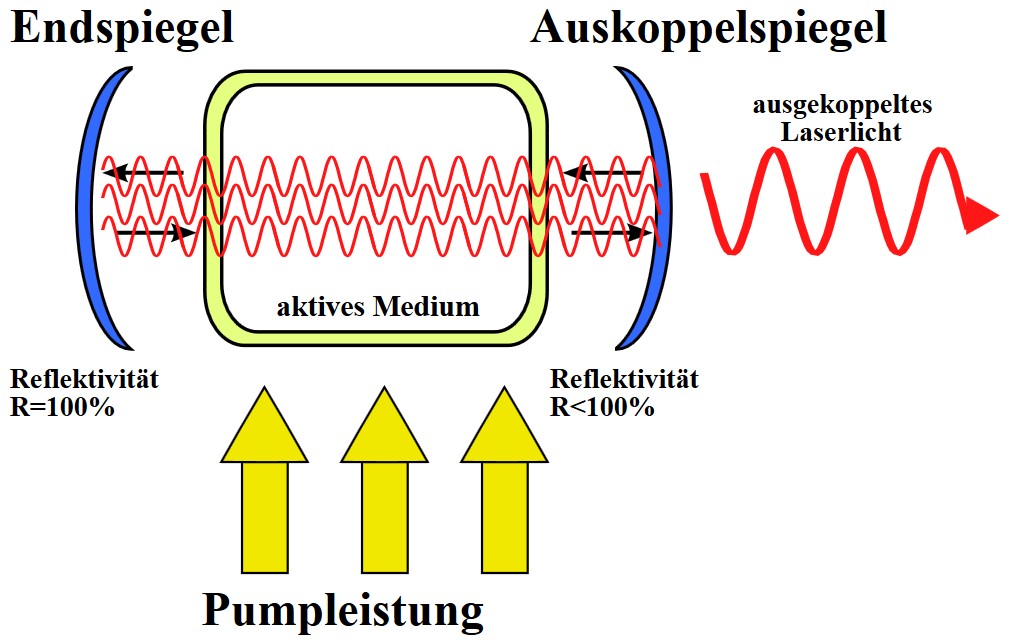
\includegraphics[scale=0.2]{img/HNL3.png}
\caption{Grundaufbau eines Lasers}
\begin{center}
\end{center}
\end{figure}

\subsection{Aktives Medium und Energiepumpe}
Um einen Laser zu betreiben, muss man dafür sorgen, dass sich das Gleichgewicht zwischen Absorption und Emission zugunsten der Emission verschiebt.Um dies zu erreichen, müssen die besetzten Zustände invertiert werden:das heißt, der energetisch höhere Zustand muss stärker besetzt sein als der niedrige. Die  stimulierte Emission wird  dadurch vorherrschend. Um dies zu erreichen, braucht man ein drittes  Energieniveau, welches höher als das zweite liegt. Auf dieses Niveau werden die Elektronen dann angeregt - was man als "pumpen" bezeichnet.
Aus dem dritten Niveau gehen sie dann emissionslos in Niveau zwei über. Dort sind sie für längere Zeit stabil. Wir haben also eine Besetztungsinversion zwischen Niveau eins und zwei erzeugt. Letztlich  gehen die Elektronen dann durch spontane Emission eines Photons zurück in den Grundzustand über. Das emittierte Photon hat dadurch allerdings  genau die Wellenlänge, die zur stimulierten Emission benötigt wird.  Dadurch wird eine Lawine von stimulierten Emissionen ausgelöst, die  schnell eine große Zahl kohärenter Photonen emittiert. Dieser Effekt  wird Superfluoreszenz genannt.

\begin{figure}[here]
\centering
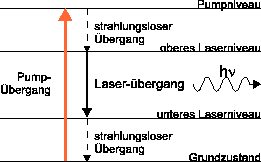
\includegraphics[scale=0.9]{img/HNL4}
\caption{Energieniveaus und Übergänge des 3-Niveau-Lasers}
\begin{center}
\end{center}
\end{figure}

\subsection{Der optische Resonator}

Der Superfluoreszenzeffekt muss für einen niedrigen Laser erweitert werden. Dazu muss das Aktive Medium in die dritte Grundkomponente eingeschlossen sein: den optischen Resonator. Dieser besteht im einfachsten Fall aus zwei hoch reflektierenden dielektrischen Spiegeln, wobei einer minimal teildurchlässig ist. Die emittierten  Photonen werden durch die Spiegel in das aktive Medium zurück reflektiert und erzeugen so noch mehr stimulierte Emissionen. Parallel dazu muss zur Aufrechterhaltung der Besetzungsinversion permanent "gepumpt" werden. Ein Teil der Photonen tritt aus dem teildurchlässigen Spiegel aus und bildet den Laserstrahl. Der Abstand der Spiegel des Resonators muss auf die jeweilige emittierte Wellenlänge angepasst sein, damit sich bei mehrmaligem Durchgang durch  die Resonanzkammer keine destruktiven Interferenzen ergeben. Der Abstand bestimmt dabei welche Wellenlängen (sog. Moden) möglich sind.
Ein weiterer wichtiger Punkt ist die Wahl der Spiegel. Auf Grund der besseren Justierbarkeit und der verringerten Beugungsverluste verwendet man häufig leicht gekrümmte Spiegel mit den Krümmungsradien $R_1$ und $R_2$. 

\begin{figure}[here]
\centering
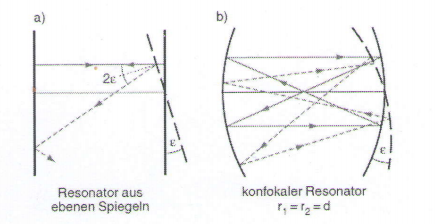
\includegraphics[scale=0.7]{img/HNL5}
\caption{Vergleich zwischen planaren (a) und gekrümmten Spiegeln (b)}
\begin{center}
\end{center}
\end{figure}

\newpage
Die Frequenz der erlaubten Moden ist wie folgt gegeben:

\begin{equation}
\nu_{qmn}=\frac{c}{2d}\left[q+\frac{m+n+1}{\pi} arccos\left(\sqrt{\left(1-\frac{d}{R_1}\right)\left(1-\frac{d}{R_2}\right)}\right)\right]
\end{equation}

Hierbei ist d die Länge des Resonators und q, m, n sind die Ordnungen der transversalen bzw. longitudinalen Moden. Die Frequenz ist reell, wodurch sich automatisch folgende logische Einschränkungen ergeben:

\begin{align}
0\leq \frac{d}{R}\leq 1 \hspace{2cm} \sqrt{\left(1-\frac{d}{R_1}\right)\left(1-\frac{d}{R_2}\right)}\leq 1
\end{align}
 
\begin{figure}[here]
\centering
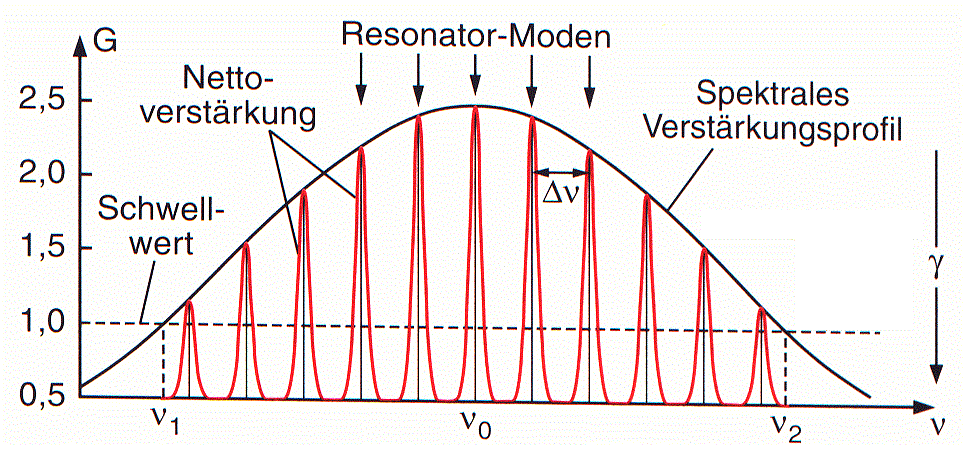
\includegraphics[scale=0.4]{img/HNL6}
\caption{Verstärkungsprofil des Resonators}
\begin{center}
\end{center}
\end{figure}

\subsection{Der Helium-Neon-Laser}
Der Helium-Neon-Laser ist ein Vier-Niveau-Laser. Das aktive Medium ist  hier eine Gasentladungsröhre, die mit Helium und Neon gefüllt ist (siehe  Abb. 5). Die Enden der Röhre sind im Brewsterwinkel angewinkelt, sodass nur ein minimaler Anteil von diesen reflektiert wird. Die Energieniveaus sind in Abb. 6 dargestellt. Durch Elektronenstöße wird das Helium vom $1^1S$ in den $2^1S$ und den $2^2S$ Zustand gepumpt. Die Heliumatome geben daraufhin durch Stöße ihre gesamte Energie an die Neon-Atome ab, die dadurch in den 3S bzw. 2S Zustand angeregt werden. Durch stimulierte Emission durchlaufen diese dann mehrere optische Übergänge. Der Hauptanteil der Übergänge liegt jedoch bei Photonen mit einer Wellenlänge von 633nm. Letztlich geht das Neon durch Stöße mit der Außenwand oder mit anderen Atomen wieder in seinen Grundzustand über.

\begin{figure}[here]
\centering
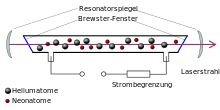
\includegraphics[scale=0.7]{img/HNL7}
\caption{Aufbau des Helium-Neon-Lasers}
\begin{center}
\end{center}
\end{figure}

\begin{figure}[here]
\centering
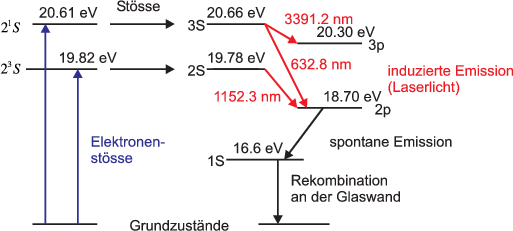
\includegraphics[scale=0.4]{img/HNL8}
\caption{Energie-Schema des Helium-Neon-Lasers}
\begin{center}
\end{center}
\end{figure}

\subsection{Linienbreite des Laserspektrums}
Da Laserlicht auf diskrete Übergänge zurückzuführen ist, müsste die natürliche Linienbreite sehr klein sein. Man beobachtet jedoch eine vielfältige Modenstruktur. Der Grund dafür, sind die Doppler- und die Stoßverbreiterung. Erstere entsteht durch die Bewegung der Gasatome. Nimmt man eine Maxwell-Boltzmann-Geschwindigkeitsverteilung der Gasatome an, so ergibt sich eine Verbreiterung von:

\begin{equation}
\Delta \nu_D = \frac{\nu_0}{c}\sqrt{\frac{8k_BT\cdot ln 2}{m}}
\end{equation}

Die Stoßverbreiterung spielt vor allem bei dichten Gasen und höheren Temperaturen eine Rolle. Hier werden die Atome allein durch thermische  Stöße gezwungen den emittierenden Energieübergang vorzeitig auszuführen. Die dadurch verkürzte Lebenszeit des Zustandes hat nach der Zeit-Unschärfe-Relation eine erhöhte Energieunschärfe zur Folge:

\begin{equation}
\Delta \nu_S = \frac{1}{2\pi \Delta \tau}
\end{equation}

Bei uns ist jedoch $\Delta \nu_D \gg \Delta \nu_S$